\section{Vista Lógica}

\begin{figure}[H]
    \centering
    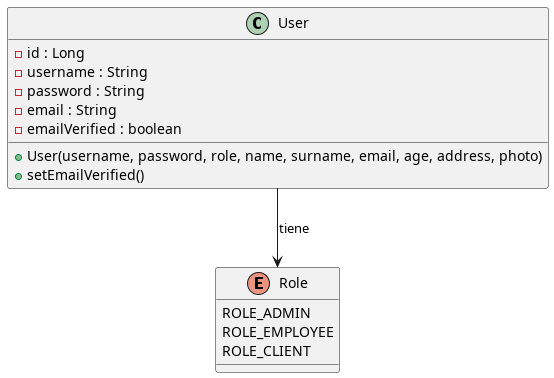
\includegraphics[width=0.5\textwidth]{img/diagrama_de_clases_user}
    \caption{Diagrama de Clases: Usuarios}
    \label{fig:dc1}
\end{figure}

La entidad \texttt{User} representa a cualquier persona que utiliza el sistema
(estudiante/cliente, personal del comedor o encargado). Contiene los datos de
identidad y autenticación (email, contraseña) y se asocia a un único
\texttt{Role}, que indica el tipo de usuario y, por lo tanto, los permisos que
posee. El enum \texttt{Role} distingue entre usuarios administradores
(\texttt{ROLE\_ADMIN}), empleados del comedor (\texttt{ROLE\_EMPLOYEE}) y
clientes finales (\texttt{ROLE\_CLIENT}). A partir de este rol, la capa de
seguridad aplica las políticas de autorización para acceder a los distintos
casos de uso del sistema.


\begin{figure}[H]
    \centering
    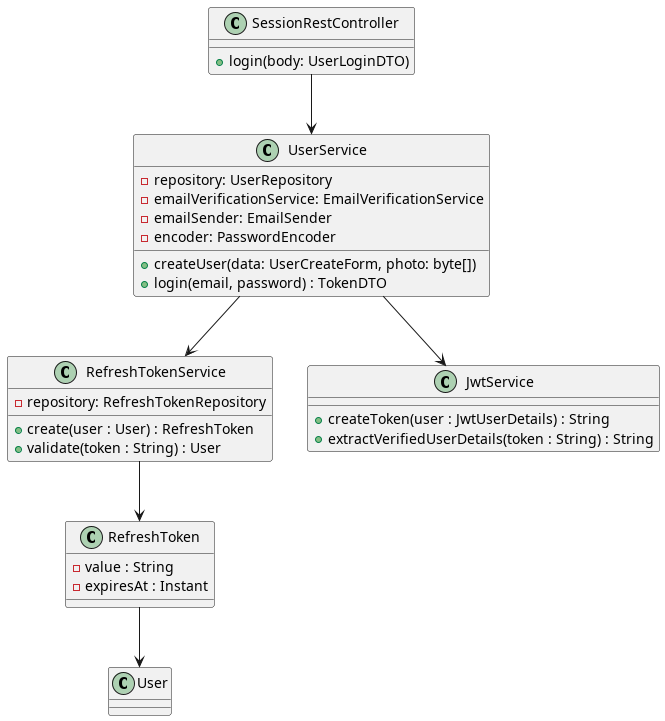
\includegraphics[width=0.7\textwidth]{img/diagrama_de_clases_user_sessions}
    \caption{Diagrama de Clases: Autenticacion de usuarios}
    \label{fig:dc1_auth}
\end{figure}

El subsistema de autenticación se organiza alrededor de \texttt{UserService},
que concentra la lógica de inicio de sesión y refresco de tokens. El
\texttt{SessionRestController} expone los endpoints HTTP de \texttt{login} y
\texttt{refresh} y delega el trabajo en dicho servicio. A partir de las
credenciales recibidas, \texttt{UserService} valida al \texttt{User}, genera
un token de acceso JWT mediante \texttt{JwtService} y un token de refresco
persistido como \texttt{RefreshToken} a través de \texttt{RefreshTokenService},
devolviendo ambos en un \texttt{TokenDTO}. De esta forma, el cliente puede
autenticarse usando JWT y renovar su sesión sin reenviar la contraseña.

\begin{figure}[htbp]
    \centering
    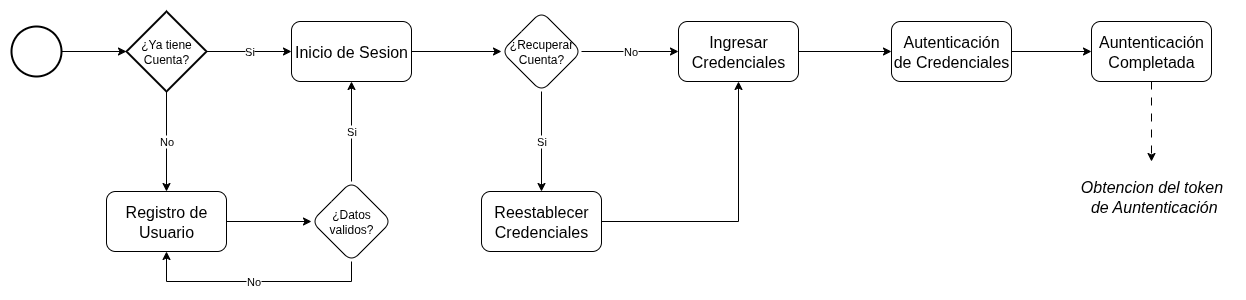
\includegraphics[width=1\textwidth]{img/Diagrama-de-estados-auth}
    \caption{Diagrama de Estados: Autenticacion de un Cliente}
    \label{fig:de2}
\end{figure}

\vfill

\begin{figure}[htbp]
    \centering
    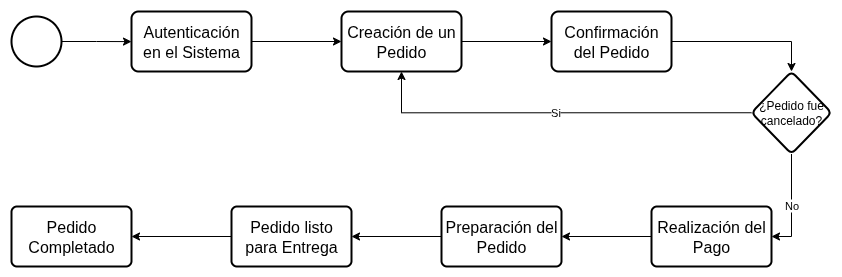
\includegraphics[width=1\textwidth]{img/Diagrama-de-estados-flujo-cliente}
    \caption{Diagrama de Estados: Flujo de un Cliente}
    \label{fig:de1}
\end{figure}

\vfill
\begin{figure}[htbp]
    \centering
    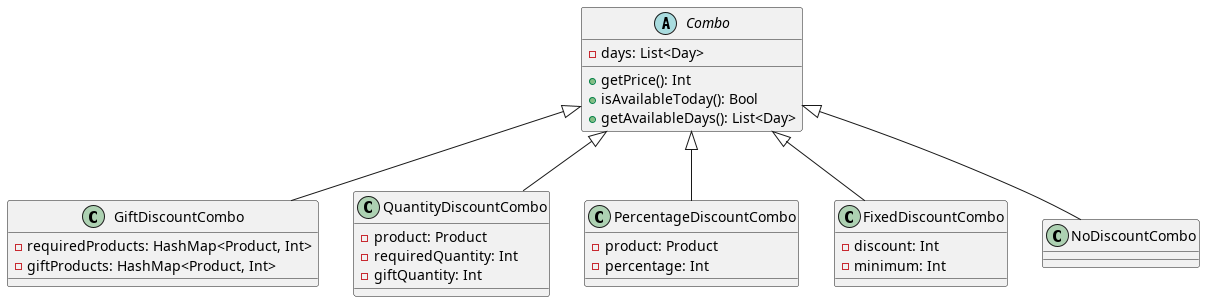
\includegraphics[width=1\textwidth]{img/diagrama_de_clases_productos}
    \caption{Diagrama de Clases: Combos y Productos}
    \label{fig:dc2}
\end{figure}
\vfill

\begin{figure}[H]
    \centering
    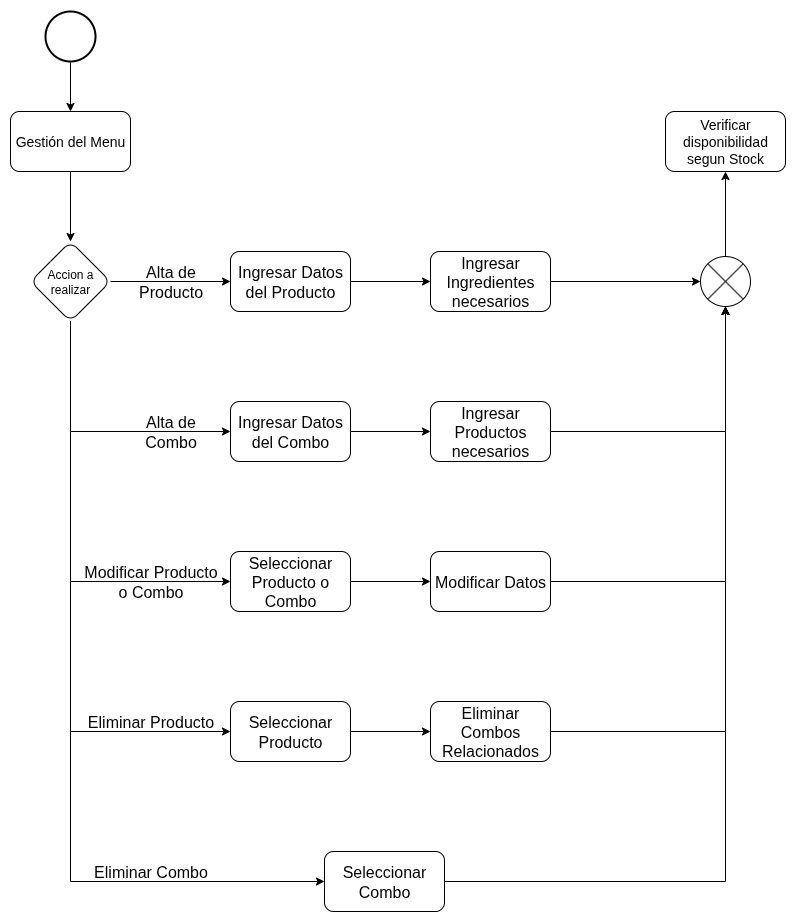
\includegraphics[width=0.7\textwidth]{img/Diagrama-de-estados-productos}
    \caption{Diagrama de Estados: Productos}
    \label{fig:de3}
\end{figure}

El siguiente diagrama modela la lógica de stock y precios del sistema. La interfaz
\texttt{Stockable} abstrae a cualquier elemento cuya disponibilidad pueda consultarse,
mientras que \texttt{Priceable} representa a los elementos que tienen un precio asociado.
\texttt{OrderItem} es una clase abstracta que unifica el comportamiento de los ítems que
pueden formar parte de un pedido (productos y combos), exponiendo operaciones para conocer
su precio, verificar disponibilidad y obtener los ingredientes que consumen. Los
\texttt{Product} se componen de uno o más \texttt{Ingredient}, que son quienes mantienen
el stock físico (\texttt{quantity}), y los \texttt{Combo} se componen de varios
\texttt{Product}. De esta forma, la disponibilidad de productos y combos se calcula siempre
en función del stock real de los ingredientes.

\begin{figure}[H]
    \centering
    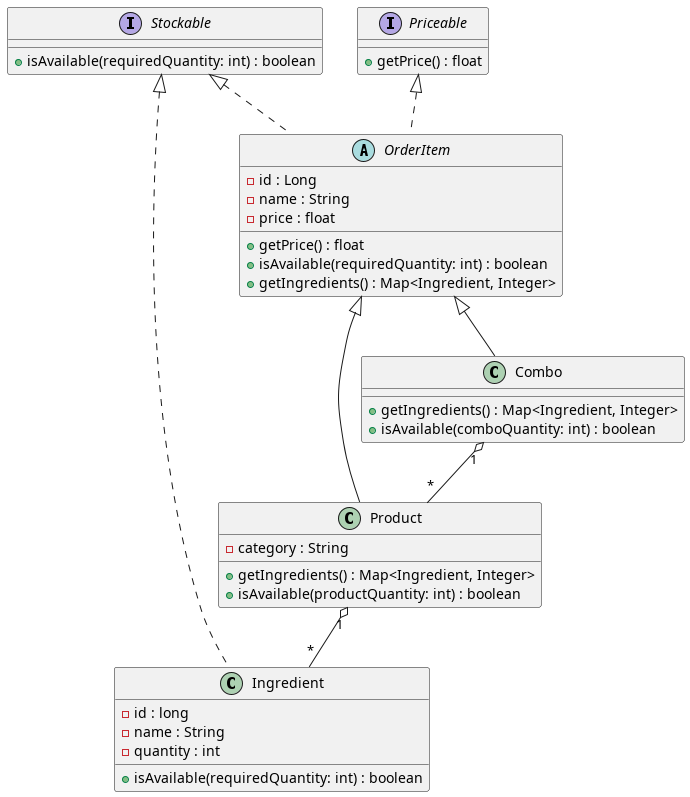
\includegraphics[width=0.4\textwidth]{img/diagrama_de_clases_stock}
    \caption{Diagrama de Clases: Stock}
    \label{fig:dc3}
\end{figure}


\begin{figure}[htbp]
    \centering
    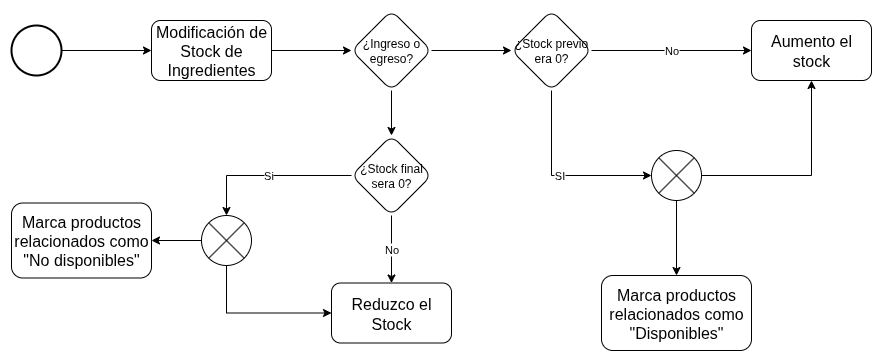
\includegraphics[width=1\textwidth]{img/Diagrama-de-estados-Gestion-de-stock}
    \caption{Diagrama de Estados: Stock}
    \label{fig:de4}
\end{figure}

\vfill
\begin{figure}[htbp]
    \centering
    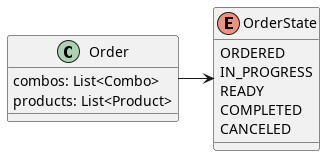
\includegraphics[width=0.4\textwidth]{img/diagrama_de_clases_estado_de_una_orden}
    \caption{Diagrama de Clases: Estados de una Orden}
    \label{fig:dc4}
\end{figure}
\vfill

\newpage
